\section{Investigation}
\label{sec:investigation}

To investigate reciprocal sharing opportunity in real life scenarios, we
obtained a \wifi{} scan result dataset from
\PhoneLab{}\footnote{\url{http://www.phone-lab.org}} (\S\ref{subsec:phonelab}).
We first discuss some heuristics to identify the home AP for each device
(\S\ref{subsec:homeap}). Then we show the RSSI comparison between a user's
home and neighbor APs (\S\ref{subsec:better}). Finally, we explore the
reciprocal sharing relationships in the dataset (\S\ref{subsec:reciprocal}).

\subsection{PhoneLab \wifi{} Dataset}
\label{subsec:phonelab}

\begin{table}[t]
  \begin{tabularx}{\columnwidth}{Xr}
    \toprule
    Begin & 11/7/2014 \\ 
    End & 4/3/2015 \\ 
    Duration (Days) & 147 \\ \midrule
    Participants & 254 \\
    Device Type & Nexus~5 \\ \midrule
    Scans & \num{21192417} \\
    Observed APs & \num{1197522} \\
    Used APs & \num{15668} \\ \midrule
    \wifi{} Sessions & \num{466032} \\
    \bottomrule
  \end{tabularx}
  \caption{\textbf{\PhoneLab{} \wifi{} Dataset Summary.} Used APs refers to the
  subset of total APs that were used by the devices participating in the study.}
  \label{tab:summary}
\end{table}

\PhoneLab{}\cite{phonelab-sensemine13} is a public smartphone platform
testbed operated at the University at Buffalo. Several hundreds of
participants carry instrumented Nexus 5 smartphones as their primary device.
In particular, the smartphone platform was modified to log each \wifi{} scan
result and \wifi{} connection events naturally generated by the Android
system. Note that from data collection point of view, platform
instrumentation is not necessary, and the same information can also be logged
by applications with appropriate permissions. A \wifi{} scan result
represents the device's network visibility, and consists of multiple
entries---each corresponds to one \wifi{} AP the device observed. The content
of one entry includes: (1) beacon timestamp, (2) AP SSID and BSSID, (3) AP
channel and (4) RSSI. The timestamp when the scan was performed is also
logged. Table~\ref{tab:summary} summarizes the \PhoneLab{} \wifi{} dataset.

\subsection{Home AP Detection}
\label{subsec:homeap}

We focus on home \wifi{} networks which are more likely to reveal stable and
immediate reciprocal sharing opportunities. For this purpose, we first developed
several heuristics to identify the home AP for each device in the dataset. The
intuition is that the devices are most likely connected to their home AP at
night. More specifically, to identify the home AP for a device, we look at
\wifi{} sessions that happened during 12~AM and 4~AM and count the number of
days that the device connects to each AP during this time period. We then
identify the AP which has the largest day count as the device's home AP,
provided that the day count is larger than a threshold (30 days) to further
filter out false positives.

After applying the above heuristics, the home AP information of 107 devices are
identified, including 101 unique BSSIDs. There are 6 BSSIDs that are identified
as home APs for two devices. After further investigation and clarification with
\PhoneLab{} administrators, we found this is because some participants are family
members, and certain participants had device replacements during the data
collection period. In both cases, multiple devices may be associated with the
same home AP.

\subsection{\wifi{} Session Signal Strength}
\label{subsec:better}

After identifying the home AP for each device, we ask two questions: (1) When
the device is connected to its home AP, how often does it receive a better signal
from neighbors' APs which it does not have access to? and (2) When the home AP
fails to provide the best signal, are there dominant neighbor APs
that provide better signal most of the time?

\sloppy{%
  To answer the first question, we inspect scan results that are reported during
  \wifi{} sessions with home APs. For each such scan result, we identify the
  currently associated home AP, $AP_{home}$, and the AP with best RSSI, denoted
  as $AP_{best}$. We are particularly interested in \textit{sub-optimal} cases,
  where: (1) $AP_{home} \neq AP_{best}$ and (2) the device never connects to
  $AP_{best}$ in the dataset. Such cases indicate that the device could
  potentially improve its \wifi{} performance by connecting to a neighbor AP
  which has a strong signal yet it does not have access to that AP. Note that
  here we consider RSSI as a hint in determining the \textit{optimal} AP and it
  is well understood that RSSI does not directly translate to \wifi{}
  performance, which we will discuss in Section~\ref{subsec:monitoring}.  Also note
  that the cases when the device is not connected to APs with the strongest
  signal due to bad roaming strategies are not interesting in the context of
  this paper, and are excluded by the second condition.
}

\begin{figure}[t]
  \centering
  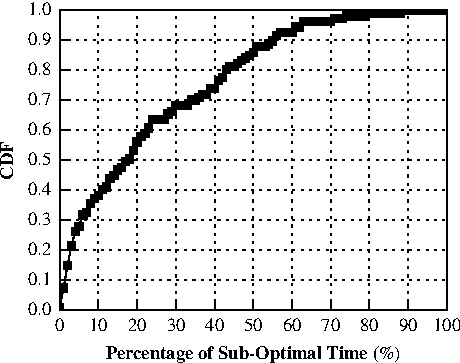
\includegraphics[width=\columnwidth]{./figures/HomeAPSessionRSSI.pdf}
  \caption{\textbf{CDF of Sub-Optimal Connection Time.}}
  \label{fig:suboptimal}
  \vspace*{-4mm}
\end{figure}

We classify all scan results reported during home \wifi{} sessions into
two categories: sub-optimal and the rest. For each device, we calculate the
percentage of time when the scan results indicate sub-optimal association.
Figure~\ref{fig:suboptimal} shows the CDF of this percentage for 
the 107 devices. We make several observations. First, for 60\% of the devices,
their home APs usually provides best signal (sub-optimal percentage less than
20\%). This result is not particularly surprising considering that home APs are
usually carefully positioned to provide good coverage. Second, we notice
that for certain number (15\%) of devices, their home APs failed to provide best
signal for more than 50\% of the time, suggesting that these users may benefit
from sharing the \wifi{} access of neighbor APs.

Next, we want to answer the question when the device is in a sub-optimal association
with its home AP, are there \textit{dominant} neighbor APs that
usually provide the best signal among other neighbor APs? If such dominant
neighbor APs exist, then by just sharing access of several particular neighbor
APs, the device's sub-optimal association time can be largely reduced. To this
end, we look at all the scan results in the sub-optimal category, and count the
number of times that each neighbor AP appears as $AP_{best}$. For each device,
we calculate the fraction of the top $n (1 \le n \le 3)$ dominant neighbor APs.
Figure~\ref{fig:dominantap} shows the CDF of dominant AP fraction. By sharing 1,
2 or 3 neighbor APs, half the device's sub-optimal connection time can be
reduced by 55\%, 82\% and 90\% respectively.

\begin{figure}[t]
  \centering
  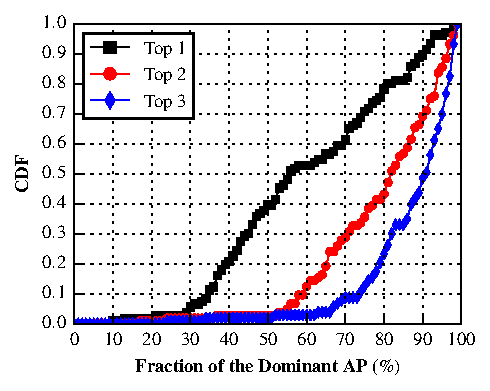
\includegraphics[width=\columnwidth]{./figures/DominantNeighborAPFigure.pdf}
  \caption{\textbf{CDF of Dominant AP Fraction.}}
  \label{fig:dominantap}
  \vspace*{-4mm}
\end{figure}

\subsection{Reciprocal Sharing Opportunities}
\label{subsec:reciprocal}

Finally, we investigate the cases where two devices can obtain better signals
from each other's home AP, i.e., reciprocal sharing opportunities. For this
purpose, we build a reciprocal sharing graph $G_r=(V, E)$, where $V$ is the set
of APs, and $\langle AP_i \rightarrow AP_j \rangle \in E$ if $AP_i$'s clients
receive better signal from $AP_j$, that is, $AP_j$ appears as $AP_{best}$ in the
scan results of $AP_i$'s clients. Note that according to the definition, $AP_i$
is one of the identified home APs, while $AP_j$ could be other arbitrary APs.
Loops in $G_r$ represent reciprocal sharing opportunities.

To capture the reciprocal sharing relationships among \PhoneLab{} participants,
we further construct a subgraph of $G_r$, $G_r'=(V', E')$, where $\langle AP_i
\rightarrow AP_j \rangle \in E'$ only if both $AP_i$ and $AP_j$ are identified
home APs of \PhoneLab{} participants. Figure~\ref{fig:reciprocal} visualize
$G_r'$, where nodes without outgoing edges are omitted for clarity. Sharing
opportunities are sparse but exist. In particular, we observe one pair of home
APs, node 0 and 7, which exhibit reciprocal sharing relationships.

\begin{figure}[t]
  \centering
  \begin{subfigure}{\columnwidth}
    \centering
    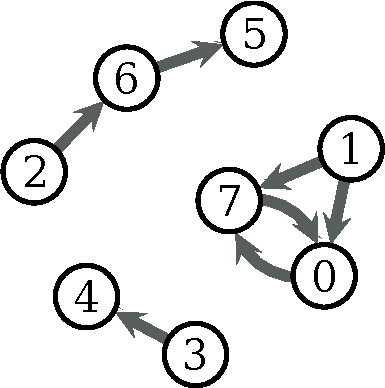
\includegraphics[width=0.5\columnwidth]{./figures/ReciprocalSharingFigure.pdf}
    \caption{\textbf{Reciprocal Sharing Graph Among PhoneLab Participants.}}
    \label{fig:reciprocal}
  \end{subfigure}
  \begin{subfigure}{\columnwidth}
    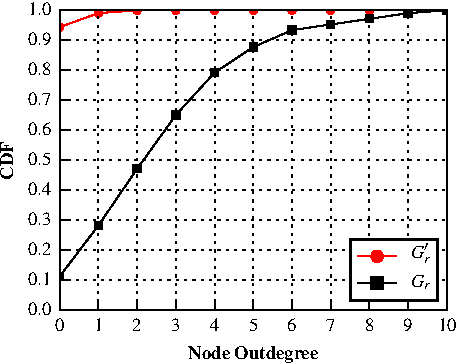
\includegraphics[width=\columnwidth]{./figures/SpatialSparseFigure.pdf}
    \caption{\textbf{CDF of Node Outdegree in Reciprocal Sharing Graph.} Only
    outdegrees of identified \PhoneLab{} home APs are counted. }
    \label{fig:sparse}
  \end{subfigure}
\end{figure}

We must point out that \PhoneLab{} participants reside sparsely among the vast
Buffalo area, and the above analysis is further restricted to those participants
that we can detect their home APs using heuristics described
Section~\ref{subsec:homeap}. The consequence of such sparsity is that most of
the neighbor APs which can provide better signal are not one of the identified
home APs, thus are not shown in Figure~\ref{fig:reciprocal}. To quantify the
spatial sparsity, Figure~\ref{fig:sparse} shows the CDF of node outdegree
in $G_r$ and $G_r'$. While the median node outdegree in $G_r$ is 2, 95\% of nodes
in $G_r'$ has no outgoing edges.  The fact that reciprocal sharing
opportunities exist at all in such a sparse dataset is quite surprising, and
motivates the need for a system to detect and enable such reciprocal \wifi{}
sharing.



